%!TEX root = ../thesis.tex
% ******************************* Thesis Appendix B ****************************
\cleardoublepage
\chapter{Dissimilarity measures between probability distributions}
\label{apx:B}
%*******************************************************************************

Beyond the discrepancy measure to the uniform distribution presented in Section~\ref{sec:central_propagation}, this Appendix introduces two families of measures commonly used to quantify the dissimilarity between two probability distributions $\pi$ and $\zeta$.  


%============================================================%
%============================================================%
\section*{Csiz\'{a}r $f$-divergences}
%============================================================%
%============================================================%

The general definition of the ``$f$-divergence'' of $\pi$ from $\zeta$, also called Cisz\'{a}r $f$-divergence after the seminal work of \citet{csiszar_1964}, is given by: 
\begin{equation}
    D_{f}\left(\pi || \zeta\right) = \int_{\Omega} f\left(\frac{\dd \pi}{\dd \zeta}\right) \, \dd \zeta, 
\end{equation}
with $f(\cdot)$ and convex function such that $f(1)=0$, and where $\pi$ is absolutely continuous w.r.t. $\zeta$. 
Let us recall some well-know divergences which are special cases of $f$-divergences:
\begin{itemize}
    \item Kullback–Leibler \citep{kullback_1951}: $f(t)=t \, \ln(t)$;
    \item Hellinger of order $\alpha \in \R_+ \textbackslash \{1\}$ \citep{jeffreys_1946}: $f(t)=(1 - \sqrt{t})$;
    \item Total variation: $f(t)= \frac12 \, |t-1|$.
\end{itemize} 
The reader may refer to \citet{basu_2011} for further details on $f$-divergences.


%============================================================%
%============================================================%
\section*{Integral probability metrics}
%============================================================%
%============================================================%

Another family of dissimilarity measures between probability distributions called the ``integral probability metrics'' (\abv{ipm}) \citep{muller_1997_ipm}, is defined as: 
\begin{equation}
    \gamma_{\iH}(\pi, \zeta) = \sup_{g \in \iH} \left | \int_{\iD_{\bX}} g(\bx) \dd \pi(\bx) - \int_{\iD_{\bX}} g(\bx) \dd \zeta(\bx) \right|,
    \label{eq:ipm}  
\end{equation}
where $\iH$ is a class of measurable functions on $\iD_{\bX} \subset \R^d$ that sets the type of IPM.   
For example, the total variation distance considers all the functions with value in $[-1, 1]$; 
furthermore, the Wasserstein distance relies on a class of Lipschitz functions; 
then a kernel-based distance called the ``maximum mean discrepancy'' (MMD) uses a specific Hilbert space. 

Between the wide panel of distances\footnotemark, a particular focus is dedicated in this section to the MMD. 
This distance was successfully use in diverse contexts for the consistency of its estimators, and its closed-form expression (even allow exact computation is some cases) \citep{sriperumbudur_2012}. 

\footnotetext{See the ``Taxonomy of principal distances and divergences'' proposed by F. Nielsen in: \\ \url{https://franknielsen.github.io/Divergence/Poster-Distances.pdf}}



%------------------------------------------------------------%
\subsection*{Kernel discrepancy}
%------------------------------------------------------------%

This section first introduces a kernel-based discrepancy called the maximum mean discrepancy, generalizing the concept of discrepancy to non-uniform measures.

\paragraph{Reproducing kernel Hilbert space and kernel mean embedding}
%------------------------------------------------------------%
Let us first assume that the function $g$ belongs in a specific function space $\iH(k)$. 
$\iH(k)$ is a \emph{reproducing kernel Hilbert space} (RKHS), which is an inner product space of functions $g:\iD_{\bX} \rightarrow \R$. 
Considering a symmetric and positive definite function $k: \iD_{\bX} \times \iD_{\bX} \rightarrow \R$, later called a ``reproducing kernel'' or simply a ``kernel'', an RKHS verifies the following axioms: 
\begin{itemize}
    \item The ``feature map'' $\phi : \iD_{\bX} \to \iH(k); \phi(\bx) = k(\cdot, \bx)$ belongs to the RKHS: $k(\cdot, \bx) \in \iH(k), \forall \bx \in \iD_{\bX}$;
    \item The ``reproducing property'': $\langle g, k(\cdot, \bx) \rangle_{\iH(k)} = g(\bx), \quad \forall \bx \in \iD_{\bX}, \forall g \in \iH(k)$.
\end{itemize}
Note that it can be shown that every positive semi-definite kernel defines a unique RKHS (and vice versa) with a feature map $\phi$, such that $k(\bx, \bx') = \langle \phi(\bx), \phi(\bx') \rangle_{\iH(k)}$.
This framework allows us to embed a continuous or discrete probability measure in an RKHS, as illustrated in \fig{fig:kernel_mean_embedding}. 
For any measure $\pi$, let us define its \emph{kernel mean embedding} \citep{sejdinovic_2013}, also called ``potential'' $P_{\pi}(\bx)$ in \cite{pronzato_zhigljavsky_2020}, associated with the kernel $k$ as:

\begin{equation}
   P_{\pi}(\bx) := \int_{\iD_{\bX}} k(\bx, \bx') \dd \pi(\bx').
\end{equation}

Respectively, the potential $P_{\zeta_n}(\bx)$ of a discrete distribution $\zeta_n = \sum_{i=1}^{n} w_i \delta(\bx^{(i)}), w_i \in \R$ associated with the kernel $k$ can be written as:
\begin{equation}\label{eq:potential}
    %P_{\pi}(\bx) := \int_{\iD_{\bX}} k(\bx, \bx') \d \pi(\bx'), \qquad 
    P_{\zeta_n}(\bx) =  \int_{\iD_{\bX}} k(\bx, \bx') \dd \zeta_n(\bx') = \sum_{i=1}^{n} w_i k(\bx, \bx^{(i)}).
\end{equation}
The potential $P_{\pi}(\bx)$ of the targeted measure $\pi$ will be referred to as ``target potential'' and the potential $P_{\zeta_n}(\bx)$ associated with the discrete distribution $\zeta_n$ called ``current potential'' when its support is the current design $\bX_n$. 
When $P_{\zeta_n}(\bx)$ is close to $P_{\pi}(\bx)$, it can be interpreted as $\zeta_n$ being an adequate quantization or representation of $\pi$. %(which leads to a good estimation of a quantity such as $I_{\pi}(g)$ from \eq{eq:quadrature_rule}). 
Potentials can be computed in closed forms for specific pairs of distribution and associated kernel. 
Summary tables of some of these cases are detailed in \cite[Sec. 3.4]{briol_phd_2019}, \cite[Sec. 4]{pronzato_zhigljavsky_2020}, and extended in \cite{fekhari_iooss_2023}. 
However, in most cases, the target potentials must be estimated on a large and representative sample, typically a large quasi-Monte Carlo sample of $\pi$.


The \emph{energy} of a measure $\pi$ is defined as the integral of the potential $P_\pi$ against the measure, which leads to the following scalar quantity:
\begin{equation}
    \varepsilon_\pi:= \int_{\iD_{\bX}} P_{\pi}(\bx) \dd \pi(\bx) = \iint_{\iD_{\bX}^2} k(\bx, \bx')\, \dd\pi(\bx) \dd\pi(\bx').
\end{equation}
\label{eq:target_energy}

\begin{figure}
    \centering
    \begin{tikzpicture}[thick, scale=0.7, every node/.style={transform shape}]
    % Axes
    \def\x{6}\def\y{3.5}
    \draw[-] (-0.5,0) -- (\x+0.5,0) node[right] {};
    \draw[-] (0,-0.5) -- (0,\y+0.5);

    \node (A) at (1.5, 3) {};
    \node (B) at (3.5, 1) {};
    \node (C) at ($(A)!0.5!(B)$) {};
    \draw[{|-|}, very thick] (A) -- (B);

    \fill [red!80] (A) circle (2pt) node[above, black] {$P_{\pi}$};
    \fill [red!80] (B) circle (2pt) node[below, black] {$P_{\zeta}$};
    \node (MMD) at (4.5, 3.5) {$\left\lVert P_{\pi} - P_{\zeta}\right\lVert_{\iH(k)}$};
    \draw[-stealth] (MMD) to [bend left] (C);

    \node [inner sep=0pt] (disc) at (-2,0.9) {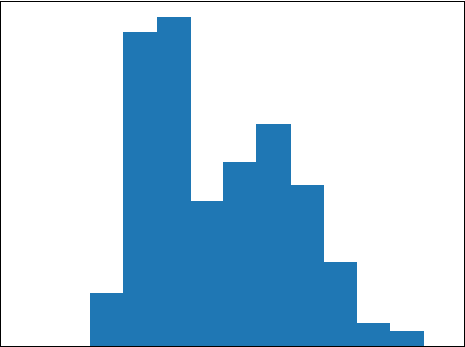
\includegraphics[width=.2\textwidth]{part2/figures/DCE/discrete.pdf}};
    \node [inner sep=0pt] (cont) at (-2,3.1) {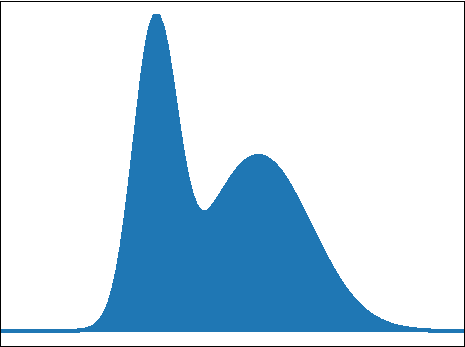
\includegraphics[width=.2\textwidth]{part2/figures/DCE/continuous.pdf}};
    \draw[-stealth] (cont) to [bend left] (A);
    \draw[-stealth] (disc.east) to [bend right] (B);
    % Text
    \node at (5, 0.25) {$\mathcal{H}_k$};
    \node at (-3, 3) {$\pi$};
    \node at (-3, 1) {$\zeta$};
\end{tikzpicture}
    \caption{Kernel mean embedding of a continuous and discrete probability distribution}
    \label{fig:kernel_mean_embedding}
\end{figure}
Finally, using the reproducing property and writing the Cauchy-Schwarz inequality on the absolute quadrature error leads to the following inequality, similar to the Koksma-Hlawka inequality \eq{eq:KH_inequality} (see \citealp{briol_oates_2019}): 

\begin{subequations}
\begin{align}
    \left| \sum_{i=1}^{n} w_i g(\bx^{(i)}) - \int_{\iD_{\bX}} g(\bx) \dd \pi(\bx) \right| &= \left| \left\langle g, P_{\zeta_n}(\bx) \right\rangle_{\iH(k)} - \left\langle g, P_{\pi}(\bx) \right\rangle_{\iH(k)} \right| \\
    &= \left| \left\langle g, \left(P_{\zeta_n}(\bx) - P_{\pi}(\bx)\right) \right\rangle_{\iH(k)} \right|\\
    &\leq \lVert g \lVert_{\iH(k)}  \left\lVert P_{\pi}(\bx) - P_{\zeta_n}(\bx) \right\lVert_{\iH(k)}.
    \label{eq:quad_error}
\end{align}
\end{subequations}

\paragraph{Maximum mean discrepancy}
%------------------------------------------------------------%
A metric of discrepancy is offered by the \emph{maximum mean discrepancy} (MMD). 
This distance between two probability distributions $\pi$ and $\zeta$ is given by the worst-case error for any function within a unit ball of the Hilbert space $\iH(k)$, associated with the kernel $k$:
\begin{equation}
    \MMD(\pi, \zeta) := %\\ 
    \sup_{\lVert g \lVert_{\iH(k)} \leq 1}
            \left | \int_{\iD_{\bX}} g(\bx) \dd \pi(\bx) - \int_{\iD_{\bX}} g(\bx) \dd \zeta(\bx) \right| %= \left\lVert P_{\pi}(\bx) - P_{\zeta}(\bx) \right\lVert_{\iH(k)}.
    \label{eq:mmd_c4}  
\end{equation}

According to the inequality in \eq{eq:quad_error}, $\MMD(\pi, \zeta) = \left\lVert P_{\pi} - P_{\zeta} \right\lVert_{\iH(k)}$, meaning that the MMD fully relies on the difference of potentials. 
Moreover, \cite{sriperumbudur_2010} defines a kernel as ``characteristic kernel'' when the following equivalence is true: $\MMD(\pi, \zeta) = 0 \Leftrightarrow \pi = \zeta$. 
This property makes the MMD a metric on $\iD_{\bX}$. 
The squared MMD has been used for various purposes such as statistical testing \citep{gretton_2006}, numerical integration \citep{chen_welling_2010}, and global sensitivity analysis \citep{daveiga_2015}. 
It can be written as follows:

\begin{subequations}
\begin{align}
    \MMD(\pi, \zeta)^2 &= \left\lVert P_{\pi}(\bx) - P_{\zeta}(\bx) \right\lVert^2_{\iH(k)}\\
        &= \left\langle \left(P_{\pi}(\bx) - P_{\zeta}(\bx) \right), \left(P_{\pi}(\bx) - P_{\zeta}(\bx) \right) \right\rangle_{\iH(k)}\\
        &= \left\langle P_{\pi}(\bx), P_{\pi}(\bx) \right\rangle_{\iH(k)} - 2 \left\langle P_{\pi}(\bx), P_{\zeta}(\bx) \right\rangle_{\iH(k)} + \left\langle P_{\zeta}(\bx), P_{\zeta}(\bx) \right\rangle_{\iH(k)}\\
        &= \iint_{\iD_{\bX}^2} k(\bx, \bx')\, \dd\pi(\bx) \dd\pi(\bx') - 2 \iint_{\iD_{\bX}^2} k(\bx, \bx')\, \dd\pi(\bx) \dd\zeta(\bx') + \iint_{\iD_{\bX}^2} k(\bx, \bx')\, \dd\zeta(\bx) \dd\zeta(\bx').
\end{align}
\end{subequations}
%Taking a discrete distribution with uniform weights $\zeta_n= \frac{1}{n} \sum_{i=1}^{n} \delta(\bx^{(i)})$, the squared MMD reduces to: 
%\begin{equation}\label{eq:mmd_design}
%    \MMD(\pi, \zeta_n)^2 = \varepsilon_\pi - \frac{2}{n} \sum_{i=1}^n P_{\pi}\left(\bx^{(i)}\right) + \frac{1}{n^2} \sum_{i, j=1}^n k\left(\bx^{(i)}, \bx^{(j)}\right).
%\end{equation}

